\chapter{Theory}
\label{Chap:theory}

% epigraph (done 2021-9-24 18:51:52)
\setlength{\unitlength}{1pt}
\setlength{\epigraphwidth}{10cm}
\epigraph{Law of physicists II: \\ Without theorists, experimentalists tend to falter. \cite{Lee:1992ui}}{--- T. D. Lee\\ \textit{History of the weak interactions (1987)}}

% goal of this chapter and structure of this chapter (done 2021-10-27 01:04:34)
This chapter mainly introduces the theory of the quantum droplet. Before that, we first briefly review the quantum scattering theory as the basis for theory of BEC and droplet. Also the scattering theory serves as basis for understanding the couple channel calculation in Chap. \ref{Chap_Feshbach}, where we fit the binding energy of the Feshbach molecule to calibrate Na-Rb molecular potential. We note here that the scattering properties play an essential role in understanding the behaviour of an ultracold sample. The second part describes the microscopic theory for two-species BEC and analytically derives its LHY correction. Then, we demonstrate the theory of droplets made of the dual-species BEC. Latter in the Chap. \ref{Chap_droplet}, we will implement both variational calculation and GPE simulation for comparing to the experiment.

\section{Quantum scattering: a short introduction}
\label{sec:quan_scat}

% introduction of this section quantum scattering (done 2021-10-24 16:59:12)
This section introduces the scattering theoretical basis of partial wave analysis as a brief reminder. In the cold atom system, due to the dilute property of the system, we only consider the two-body elastic scattering. Elastic collisions dominate many cold atom processes, including evaporative cooling, the interacting BEC, etc. Because of the low scattering energy scale of the cold atom system, we use the partial wave method and only consider the lowest partial waves, $s$-, $p$-, etc. Especially for BEC systems with interactions, s-wave is sufficient to retrieve all the elastic scattering information. This leads to the use of Pseudo-potential with the same $s$-wave scattering length to replace the real complex scattering potential, which will be further introduced in Sec. \ref{sec:droplet_ana}.

% Hamiltonian (done 2021-10-24 17:01:34)
The partial-wave method solves the stationary Schrodinger equation by separating the wave function into the different partial waves, labelled by $s-$, $p-$ and so on. The Hamiltonian of the system is
\begin{equation}
\left(-\frac{\hbar ^2}{2m}\nabla ^2+\hat{V}(r)\right)\psi _k(r,\theta ,\phi )=\psi _k(r,\theta ,\phi )
\end{equation}
separating the state into radial and angular parts
\begin{equation}
\psi _k(r,\theta ,\phi )=R_l(k.r)Y_{\text{lm}}(\theta,\phi)
\end{equation}
and then the radial part equation
\begin{equation}
\left(\frac{d^2}{dr^2}+\frac{2}{r}\frac{d}{dr}-\frac{l(l+1)}{r^2}-\frac{2m}{\hbar ^2}V(r)+k^2\right)R_l(k,r)=0
\end{equation}
Then, we already know that the form of wave function when r is very large, i.e.
\begin{equation}
\psi (r)=e^{i k z}+f(k,\theta )\frac{e^{i k r}}{r}
\end{equation}
by spherical expanding we get:
For left side:
\begin{equation}
\psi (r)=\sum _{l =0}^{\infty } R_l(k,r)P_l(\text{Cos}[\theta ])
\end{equation}
For right side:
\begin{equation}
e^{i k z}=\sum _{l=0}^{\infty}(2l+1)i^l(kr)^{-1}\text{Sin}\left[k r-\frac{l \pi }{2}\right]P_l(\text{Cos}[\theta])
\end{equation}
\begin{equation}
f(k,\theta )=\sum _{l =0}^{\infty } f_l(k)P_l(\text{Cos}[\theta ])
\end{equation}
Thus we have the Radial part with different $l$ as
\begin{equation}
R_l(k,r)=(2l+1)i^l(k r)^{-1}\text{Sin}\left[k r-\frac{l \pi }{2}\right]+f_l(k)\frac{e^{i k r}}{r}
\end{equation}
If we are treating some finite range potential, there exists a general solution:
Suppose that the potential can be written as
\begin{equation}
V(r)=\left\{
\begin{array}{c}
 V(r), r<r_0 \\
 \quad 0, r>r_0 \\
\end{array}
\right.
\end{equation}
When $r>r_0$ we have
\begin{equation}
\left(\frac{d^2}{dr^2}+\frac{2}{r}\frac{d}{dr}-\frac{l(l+1)}{r^2}+k^2\right)R_l(k,r)=0
\end{equation}
Solution of this equation has been solved well as following
\begin{equation}
R_l(k,r)=B_l(k)j_l(kr)+C_l(k)y_l(kr)
\end{equation}
When r $\to \infty $, we get the asymptotic from of Bessel function as
\begin{equation}
R_l(k,r)=\frac{1}{k r}\left\{A_l(k)\text{Sin}\left[k r-\frac{l \pi }{2}-\delta _l(k)\right]\right\}
\end{equation}
where
\begin{equation}
A_l(k)=\sqrt{B_l^2(k)+C_l^2(k)},\text{  }\delta _l(k)=\text{ArcTan}\left[\frac{C_l(k)}{B_l(k)}\right]
\end{equation}
Comparing [12] and [16], we get that
\begin{equation}
f_l(k)=\frac{2l+1}{2i k}\left[e^{2i \delta _l(k)}-1\right]
\end{equation}
\begin{equation}
A_l(k)=(2l+1)i^le^{i \delta _l(k)}
\end{equation}
Finally, we have
\begin{equation}
f(k,\theta )=\sum _{l =0}^{\infty } \frac{2l+1}{2i k}\left[e^{2i \delta _l(k)}-1\right]P_l(\text{Cos}[\theta ])
\end{equation}
Now, if we connect the boundary condition inside $r_0$, we can solve the $\delta _l(k)$ and solve this problem.
For now, we can say that if we get all $\delta _l(k)$, then we solve this problem well. Nevertheless, that is a massive project because there are infinite $l$, and for each $l$, $\delta$ is a function of k; thus, we need a good approximation for our system. Then, the last feature, low temperature, can be used. 

% add collision low energy (done 2021-10-27 01:07:50)
\begin{figure}[htb]
\begin{center}
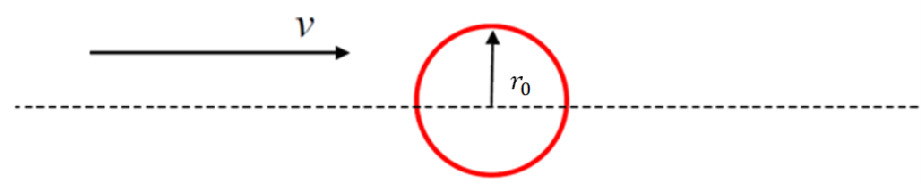
\includegraphics [width = 0.8 \linewidth]{theory_low_energy_scattering.pdf}
\end{center}
\caption[Low energy scattering of finite range potential]{shows the low-energy scattering. Only the lowest several partial wave matter.}
\label{theory_low_colli}
\end{figure}

% low energy collision (done 2021-10-27 16:29:34)
As shown in Fig. \ref{theory_low_colli}, particles can hit this finite potential with $l$ less than 
\begin{equation}
l<l_{\max }=\frac{m v r_0}{\hbar }=r_0 k
\end{equation}
where $r_0$ is the potential range. Thus, At low-energy limit, i.e. $r_0k\to 0$, we have $l_{\max }\to 0$, which means we can consider $s$-wave only.
\begin{equation}
f_0(k)=\frac{1}{2ik}\left[e^{2i\delta_l(k)}-1\right]=\frac{1}{k}e^{i \delta _0(k)}\text{Sin}\left[\delta _0(k)\right]
\end{equation}
Thus, only one parameter $\delta _0(k)$ representing whole process. As historical preference, we introduce an equivalent parameter, scattering length $a_S$
\begin{equation}
a_s=a_0(k)|_{k\to0}=\underset{k\to0}{\text{Lim}}\left[-\frac{1}{k}\text{Tan}\left[\delta _0(k)\right]\right]
\end{equation}
where $a_s$ is independent with $k$, just as what we want.
Conclusion: when we deal with finite range potential scattering, not need to be finite intensity potential, and if the particle's momentum k is so small that $k \ll 1/a$, where a is the potential range, we can use only one parameter $a_0$ to describe the whole scattering process. The approximations made here are listed below:
Finite range potential gives $r_0$.
$k \ll 1/r_0$ where k is scattering momentum divided by $\hbar$, and $r_0$ is potential range
Scattering length $a_0$ actually depends on k, however if we consider the limit $k\to 0$, we can ignore this variance.
This very beautiful property gives us a way to deal with not-weak atom-atom scattering problem even with strong interaction.

%\subsection{Resonance scattering}


\section{Quantum droplet}
\label{sec:droplet_ana}

% overall of this section (done 2021-10-27 16:41:56)
In this section, we introduce the basic theory of quantum droplets. We start from the most basic theory of BEC and first provide the treatment of BEC by Bogoliubov, which leads to the correction of ground state energy given by LHY correction. This part describes a detailed derivation than the introduction part. Subsequently, we introduce the theory of two-component BEC and obtain a numerical solution of the LHY correction in this case, which typically has no analytical solution if the mass of both species is imbalanced. Then, we explain the formation mechanism of the quantum droplet made of Bose mixture. In this subsection, we consider only the bulk sample, ignoring the kinetic energy term and finally obtain the density of a stable quantum droplet as a function of inter-species interaction. We will discuss the theory and simulation of the finite-size droplet in the Experiment Chapter \ref{Chap_droplet}.

\subsection{Dilute Bose system: Pseudo-Hamiltonian and Bogoliubov transformation}

% characterization (done 2021-10-27 16:45:55)
There are three keywords for this special system: short-range interaction, dilute and low-temperature. Short-range gives a length scale $r_0$, which represent the inter-particle potential range. Dilute means: $n^{1/3}r_0 \ll 1$, where n denote particle number density. Low temperature(energy) means $k r_0 \ll 1$, where $k$ denotes momentum. These three conditions allow us to replace the real complicated potential between atoms by a pseudo-potential. The only related parameter then is the $s$-wave scattering length $a_s$ when the temperature is low enough, as we mentioned before.

%Pseudo-potential (done 2021-10-27 16:51:21)
As we can use $a_s$ representing scattering process, we can write down a pseudo-potential, which gives the same effect as the original one. This procedure first done by \textit{Fermi} as following
\begin{equation}
V(r)=g \delta (r)\partial _r\cdot r=\frac{4\pi\hbar^2a_s}{m}\delta (r)\partial _r\cdot r
\end{equation}
which is a contact potential only affect two atoms when they have same $r$. The last term $\partial _r\cdot r$ eliminates wave function's divergence at $r\to 0$, due to it has form of $\psi \to 1-\left.a_S\right/r$. if we write the potential as
\begin{equation}
V(r)=g_R\delta (r)
\end{equation}
where $g_R$ denotes the interaction intensity. Note that this $g_R$ cannot be considered as physics quantity due to its divergence at $r\to 0$. However, the relationship between $g_R$ and $g$ can be obtain by \textit{Dyson} Equation.
\begin{equation}
g_R=g+g \Sigma ^* g_R
\end{equation}
where $g_R$ represent normalized interaction strength, and $\Sigma^*$ represent the proper self-energy of system, i.e.
\begin{equation}
g_R=\frac{4\pi  \hbar ^2a_s}{m}\left(1+\frac{g_R}{V}\sum _{k=0}^{\infty } \frac{1}{\hbar ^2\left.k^2\right/m}\right)
\end{equation}
by just take the second order correction (loop correction), we get
\begin{equation}
\label{gRRe}
g_R=g\left(1+\frac{g}{V}\sum _{k=0}^{\infty } \frac{1}{\hbar ^2\left.k^2\right/m}\right)
\end{equation}
The second term is actually diverge, which represents high energy scattering. This term will only be used when we need to sum over some term with all high energy collision process. In most time, we can just take $g$ as
\begin{equation}
g=\frac{4\pi  \hbar ^2a_s}{m}
\end{equation}

% Hamiltonian (done 2021-10-27 16:51:55)
Then, we can rewrite the whole Hamiltonian as following
\begin{equation}
\begin{split}
\hat{H}_0&=\frac{1}{2}\int \nabla \hat{\Psi }^\dagger(x)\nabla \hat{\Psi }(x)dx\\
H_1&\simeq \frac{1}{2}\int \hat{\Psi }^\dagger(x)\hat{\Psi }^\dagger(x')g \delta (x-x')\hat{\Psi }(x')\hat{\Psi }(x)dxdx'\\
&=\frac{g}{2}\int \hat{\Psi}^\dagger(x)\hat{\Psi }^\dagger(x)\hat{\Psi }(x)\hat{\Psi }(x)dx
\end{split}
\end{equation}
Fourier transformation provides the Hamiltonian in momentum space as
\begin{equation}
\label{Hamil_psuedo}
H_{\text{pseudo}}=\sum_k\epsilon_k\hat{a}_k^\dagger\hat{a}_k+\frac{g}{2V}\sum _{\left\{k_i\right\}}\hat{a}_{k_1}^\dagger\hat{a}_{k_2}^\dagger\hat{a}_{k_3}\hat{a}_{k_4}
\end{equation}
where $k_1+k_2=k_3+k_4$, satisfies momentum conservation. This is just the pseudo-Hamiltonian for many-Boson system.
Because of the special role of the state with k = 0, i.e. condensate, we separate ladder operator into two piece for whole Bose gas
\begin{equation}
\hat{\Psi }(x)=\frac{1}{\sqrt{V}}\sum _{p\neq 0} e^{i p x}\hat{a}_p+\frac{1}{\sqrt{V}}\hat{a}_0=\hat{\Psi }'(x)+\frac{1}{\sqrt{V}}\hat{a}_0
\end{equation}
\begin{equation}
\hat{\Psi }^\dagger(x)=\frac{1}{\sqrt{V}}\sum _{p\neq 0} e^{-i p x}\hat{a}_p^\dagger+\frac{1}{\sqrt{V}}\hat{a}_0^\dagger=\hat{\Psi }'^\dagger(x)+\frac{1}{\sqrt{V}}\hat{a}_0^\dagger
\end{equation}
where $\hat{a}_0=\hat{a}_0^\dagger=\sqrt{n}=\sqrt{\frac{N}{V}}$, indicating the MF condensate wave-function without the quantum fluctuation. Noticed that, when we use mean field theory to calculate a system ,we need pay attention to what kind of  fluctuation we ignored in the calculation, then at necessary time, we can get it back.

% MF solution (done 2021-10-28 10:55:51)
put them into eq. \ref{Hamil_psuedo}, then simply
\begin{equation}
\begin{split}
H=\frac{g N^2}{2V}&+\sum_{k\neq0}\left(\epsilon_k+gn_0\right)\hat{a}_k^\dagger\hat{a}_k+\frac{gN}{2V}\sum_{k\neq0}\left(\hat{a}_k^\dagger\hat{a}_{-k}^\dagger+\hat{a}_k\hat{a}_{-k}\right)\\
&+\frac{g\sqrt{N}}{2V}\sum_{k_1+k_2+k_3=0}\left(\hat{a}_{k_1}^\dagger\hat{a}_{k_2}^\dagger\hat{a}_{k_3}+\hat{a}_{k_1}^\dagger\hat{a}_{k_2}\hat{a}_{k_3}\right)+\frac{g}{2V}\sum_{k_i\neq0}\hat{a}_{k_1}^\dagger\hat{a}_{k_2}^\dagger\hat{a}_{k_3}\hat{a}_{k_4}
\end{split}
\end{equation}
Here, we drop the terms with order less than $N$, because they are much smaller than others when temperature is quite low and  large amount of atoms are condensate. ( Noted that, if considering the last two term, we will get the Beliaev-Landau Damping.)
\begin{equation}
H_{\text{pseudo}}\simeq\frac{gN^2}{2V}+\sum_{k\neq0}\left(\epsilon _k+g n_0\right)\hat{a}_k^\dagger\hat{a}_k+\frac{gn_0}{2}\sum_{k\neq0}\left(\hat{a}_k^\dagger\hat{a}_{-k}^\dagger+\hat{a}_k\hat{a}_{-k}\right)\end{equation}
Now, as quadratic form, we can diagonalize it with so called Bogoliubov transformation
\begin{equation}
\begin{split}
\hat{a}_k=u_k\hat{\alpha }_k-v_k\alpha _{-k}^\dagger\\
\hat{a}_{-k}=u_k\hat{\alpha }_{-k}-v_k\alpha _k^\dagger
\end{split}
\end{equation}
where $\alpha _k^\dagger\left(\alpha _k\right)$ is a new ladder operator, which actually denote create(annihilate) a quasi-particle in this condensate system. $u_k$ and $v_k$ is c-number as function of $k$ and $E_k$, which gives the spectrum of quasi-particle. 
Finally, we give out the diagonalized Hamiltonian as
\begin{equation}
\label{Hamil_psuedo_dia}
\begin{split}
H_{\text{pseudo}}\simeq \frac{g N^2}{2V}-\frac{1}{2}\sum _{k\neq 0} \left(\epsilon _k+\frac{g N}{V}-E_k\right)+\sum _{k\neq 0} E_k\hat{\alpha }_k^\dagger\hat{\alpha
}_k\\
E_k=\sqrt{\epsilon _k\left(\epsilon _k+\frac{2 g N}{V}\right)}=\sqrt{\frac{\hbar ^2k^2}{2m}\left(\frac{\hbar ^2k^2}{2m}+\frac{2 g N}{V}\right)}
\end{split}
\end{equation}
The gap-less linear low energy excited dispersion relation gives the super fluid property, as shown in Fig. \ref{dispersion_relation_repulsive}. when $k$ get larger, it turn back to classical particle. 

% dispersion_relation_repulsive (done 2021-10-24 22:51:17)
\begin{figure}[htb]
\begin{center}
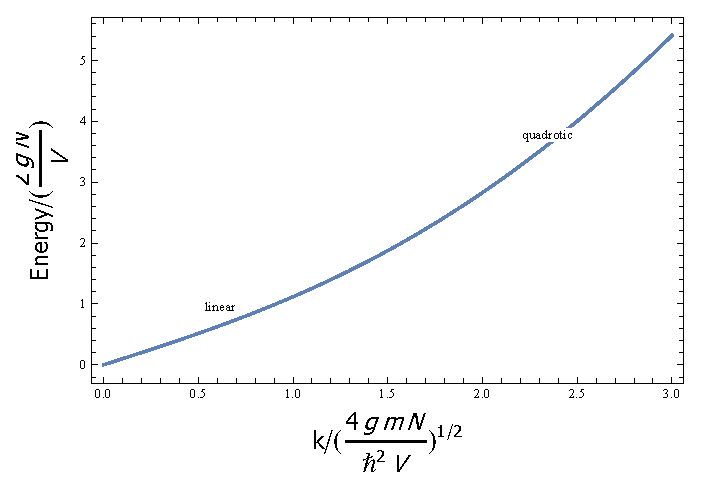
\includegraphics [width = 0.8 \linewidth]{Note for review_gr1.eps}
\end{center}
\caption[This plot shows the dispersion relationship for attractive Bose system.]{This plot shows the dispersion relation ship for quasi-particle in the Bose-condensation. When k is small, it looks like a phonon, however, when k goes large it back to a particle-like quasi-particle.}
\label{dispersion_relation_repulsive}
\end{figure}

% Negative interaction (done 2021-10-28 10:59:25)
Now, let's consider what happens when $g<0$, i.e. attractive potential between atoms. The excitation spectrum will have no low-energy excitation part, since the low-energy excitation indicates the density wave and this will cause positive feedback to increase the density of the sample, which renders the so-called collapsing of BEC. However, the high-energy excitation is still there as shown in Fig. \ref{dispersion_relation_attrac} We will argue weather this single species BEC with negative interaction can form the quantum droplet in the next subsection. 

% dispersion_relation_attrac (done 2021-10-24 22:51:17)
\begin{figure}[htb]
\begin{center}
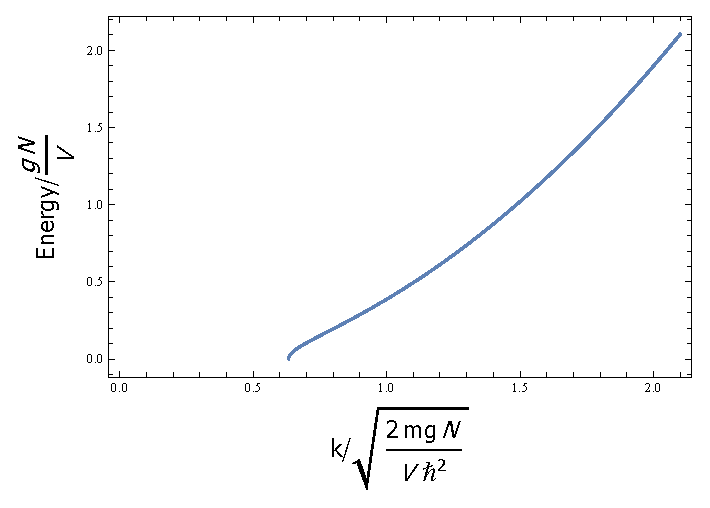
\includegraphics [width = 0.8 \linewidth]{Note for review_gr2.eps}
\end{center}
\caption[This plot shows the dispersion relationship for attractive Bose system.]{This plot shows the dispersion relationship for attractive Bose system, i.e. $g<0$.}
\label{dispersion_relation_attrac}
\end{figure}

\subsection{Ground state and the LHY correction}
% ground state (done 2021-10-28 11:03:23)
Now let us consider the ground state energy of this system. Directly take the lowest energy level from eq. \ref{Hamil_psuedo_dia}, we have
\begin{equation}
\begin{split}
E_{\text{GS}}=\frac{g N^2}{2V}-\frac{1}{2}\sum _{k\neq 0} \left(\epsilon _k+\frac{g N}{V}-E_k\right)
\end{split}
\end{equation}
where first term represent the mean field energy shift from {``}vacuum{''}, and second term come from quantum fluctuation (at zero temperature), i.e.
\begin{equation}
-\frac{1}{2}\sum _{k\neq 0} \left(\epsilon _k+\frac{g N}{V}-E_k\right)=-\frac{1}{2}\sum _{k\neq 0} \left(\frac{\hbar ^2k^2}{2m}+\frac{g N}{V}-\sqrt{\frac{\hbar
^2k^2}{2m}\left(\frac{\hbar ^2k^2}{2m}+\frac{2 g N}{V}\right)}\right)
\end{equation}
If you plot the term in the summation, you will find it decays with k increasing. However, if we expand it in series, we have 
\begin{equation}
\begin{split}
\frac{\hbar ^2k^2}{2m}&+\frac{g N}{V}-\sqrt{\frac{\hbar ^2k^2}{2m}\left(\frac{\hbar ^2k^2}{2m}+\frac{2 g N}{V}\right)}\\
&=\frac{1}{2}\left(\frac{gN}{V}\right)^2\left(\frac{2m}{\hbar^2}\right)\frac{1}{k^2}-\frac{1}{2}\left(\frac{gN}{V}\right)^3\left(\frac{2m}{\hbar^2}\right)^2\frac{1}{k^4}+\text{...}
\end{split}
\end{equation}
with leading proportional to $\frac{1}{k^2}$, we have divergence when sum over k to infinite. This divergence is due to the pseudo-potential with $\delta (r)$ actually does not allow calculation for large $k$, thus, we need do re-normalization to truncate this $\frac{1}{k^2}$ divergence.

% re-normalization (done 2021-10-28 11:05:12)
Recalling the renormalized interaction $g_R$ in eq. \ref{gRRe}, we have
\begin{equation}
g_R=g+\frac{g^2}{V}\sum _k \frac{m}{\hbar ^2k^2}
\end{equation}
Then total energy will be
\begin{equation}
\begin{split}
E_{\text{GS}}^R=\frac{gN^2}{2V}&-\frac{1}{2}\sum_{k\neq0}\left(\frac{\hbar ^2k^2}{2m}+\frac{gN}{V}\right.\\
&\left.-\sqrt{\frac{\hbar^2k^2}{2m}\left(\frac{\hbar^2k^2}{2m}+\frac{2gN}{V}\right)}-\left(\frac{gN}{V}\right)^2\left(\frac{2m}{\hbar ^2}\right)\frac{1}{k^2}\right)
\end{split}
\end{equation}
Directly do the summation, we get the famous LHY correction
\begin{equation}
\frac{E_{\text{GS}}^R}{V}=\frac{g n^2}{2}\left(1+\frac{128}{15\pi ^{1/2}} \left(n a_s^3\right)^{1/2}\right)
\end{equation}
For positive interaction strength $g>0$, we can find the LHY correction is a tiny \textit{correction} when density is low, with an order of $n a_s^3$. This has been experimentally verified in strong interacting Bose System \cite{Navon2011}. What we are interested is the case with negative interaction strength, i.e. $g<0$.The ground state energy of this case shows that there is a local minimum for a specific density. Noted that actually for $g<0$ the ground state energy formalism is ill-defined, since one cannot do the summation to get the LHY correction unless rule out the imaginary part of the low-energy excitation section. Moreover, considering the density of the local minimum, we will find that it is at the level of $n a_s^3 \approx 1$, which actually entering the strong interaction regime.

\subsection{Quantum Depletion}
% quantum depletion (done 2021-10-28 11:24:02)
Now, Let us consider a ground state of BEC at zero temperature, how many particles will not stay at $k=0$ state? The answer is that directly summing all non-zero k state in the ground state. as following
\begin{equation}
n_{\text{dp}}=\frac{1}{V}\sum _{k\neq 0} v_k^2=\frac{1}{3\pi ^2}\left(\frac{m c}{\hbar }\right)^3\propto \xi ^{-3}
\end{equation}
where $v_k$ is parameter in Bogoliubov transformation, $c =\sqrt{\frac{g n}{2m}}$ is the first sound speed in BEC, and $\xi =\frac{\hbar }{\sqrt{2m g n}}$ is healing length.
The fraction of depleted particle is
\begin{equation}
\frac{n_{\text{dp}}}{n}=\frac{8}{3\sqrt{\pi }}\sqrt{n a_s^3}
\end{equation}
we can directly read that with increasing of $n a_s^3$, more particles are kicked out of the condensate. Meanwhile, these particles will contribute an additional energy to ground state energy, i.e. the LHY correction we mentioned before.

\subsection{Mean-field theory of the Double BEC}

% introduce to double BEC case (done 2021-10-28 11:36:36)
With a brief review in several previous subsections, we found that: if there is only one species, since the LHY energy is always much smaller than MF energy, unless we increase the density or interaction strength to a strong interaction regime, the pure quantum effect always remains as a tiny correction. Therefore, only if there are some methods to maintain the LHY correction and reduce the MF energy by other effects (such as dipolar interaction or another species) can we make the MF energy scale approximate to the LHY correction. Finally, we have the opportunity to demonstrate this pure quantum effect. As Petrov mentioned in the seminal work \cite{petrov2015}: if we consider a two-species BEC sample with intra-species interaction in both positive while adjusting inter-species interaction negative enough to make almost total MF be zero, the LHY correction, since it is derived from quantum depletion, can maintain at the $g_{ii} n_i^3$ level and the MF energy can be an arbitrary proxy to zero, which form the opportunity to observe LHY correction directly. In other words, LHY correction can still exist even MF energy equals 0. In this way, it is possible to form an ultra-dilute quantum droplet since the interaction is still weak and density is actually remaining in the typical gaseous BEC level.

% Hamiltonian (done 2021-10-28 11:36:00)
Now, we turn to describe double BEC with mean field theory. Hamiltonian for BEC with two species is
\begin{equation}
\begin{split}
H_{\text{tot}}=&\sum_k\epsilon_{1,k}\hat{a}_{1,k}^\dagger\hat{a}_{1,k}+\frac{g_{11}}{2V}\sum_{\left\{k_i\right\}}\hat{a}_{1,k_1}^\dagger\hat{a}_{1,k_2}^\dagger\hat{a}_{1,k_3}\hat{a}_{1,k_4}+\sum_k\epsilon_{2,k}\hat{a}_{2,k}^\dagger\hat{a}_{2,k}\\
&+\frac{g_{22}}{2V}\sum_{\left\{k_i\right\}}\hat{a}_{2,k_1}^\dagger\hat{a}_{2,k_2}^\dagger\hat{a}_{2,k_3}\hat{a}_{2,k_4}+\frac{g_{12}}{V}\sum_{\left\{k_i\right\}}\hat{a}_{2,k_1}^\dagger\hat{a}_{1,k_2}^\dagger\hat{a}_{1,k_3}\hat{a}_{2,k_4}
\end{split}
\end{equation}
where $k_1+k_2=k_3+k_4$, satisfy momentum conservation.$g_{\text{ii}}$ represent intra-interaction strength, and $g_{12}$ for inter-interaction.
$\hat{a}_{i,k}^\dagger$($\hat{a}_{i,k}$) denote the ladder operator for $i^{\text{th}}$ component.
Because of the special role of the state with k = 0, i.e. condensate, we separate ladder operator into two piece for whole Bose gas
\begin{equation}
\begin{split}
\hat{\Psi }_i(x)=\frac{1}{\sqrt{V}}\sum_{p\neq0}e^{ipx}\hat{a}_{i,p}+\frac{1}{\sqrt{V}}\hat{a}_{i,0}=\hat{\Psi }_i'(x)+\frac{1}{\sqrt{V}}\hat{a}_{i,0}\\
\hat{\Psi }_i^\dagger(x)=\frac{1}{\sqrt{V}}\sum_{p\neq0}e^{-ipx}\hat{a}_{i,p}^\dagger+\frac{1}{\sqrt{V}}\hat{a}_{i,0}^\dagger=\hat{\Psi}'^\dagger(x)+\frac{1}{\sqrt{V}}\hat{a}_{i,0}^\dagger
\end{split}
\end{equation}
Then we get Hamiltonian as
\begin{equation}
\begin{split}
H=&\frac{g_{11}N_1^2+g_{22}N_2^2+2g_{12}N_1N_2}{2V}+\sum _{k\neq 0} \left(\epsilon_{1,k}+\frac{g_{11}N_1+g_{12}N_2}{V}\right)\hat{a}_{1,k}\dagger\hat{a}_{1,k}\\
&+\sum_{k\neq 0} \left(\epsilon_{2,k}+\frac{g_{22}N_2+g_{12}N_1}{V}\right)\hat{a}_{2,k}^\dagger\hat{a}_{2,k}+\frac{g_{11} N_1}{2V}\sum _{k\neq 0}\left(\hat{a}_{1,k}^\dagger\hat{a}_{1,-k}^\dagger+\hat{a}_{1,k}\hat{a}_{1,-k}\right)\\
&+\frac{g_{22} N_2}{2V}\sum_{k\neq0}\left(\hat{a}_{2,k}^\dagger\hat{a}_{2,-k}^\dagger+\hat{a}_{2,k}\hat{a}_{2,-k}\right)\\
&+\frac{g_{12}\sqrt{N_1N_2}}{2V}\sum _{k\neq 0} \left(\hat{a}_{1,k}^\dagger\hat{a}_{2,k}+\hat{a}_{2,k}^\dagger\hat{a}_{1,k}+\hat{a}_{1,k}\hat{a}_{2,-k}+\hat{a}_{2,k}^\dagger\hat{a}_{1,-k}^\dagger\right)
\end{split}
\end{equation}
where we only keep the second order of $N_i$, dropping third and forth order of $N_i$. Then, diagonalize this Hamiltonian by extended Bogoliubov transformation for double BEC, we have
\begin{equation}
\begin{split}
H=&\frac{g_{11}N_1^2+g_{22}N_2^2+2g_{12}N_1N_2}{2V}\\
&+\frac{1}{2}\sum _{k\neq 0} \left(E_++E_--\frac{\hbar ^2k^2}{2m_1}-\frac{\hbar ^2k^2}{2m_2}-\frac{g_{11}N_1+g_{22}N_2}{V}\right)\\
&+\sum_{k\neq 0} E_{+,k}\hat{a}_{+,k}^\dagger\hat{a}_{+,k}+\sum _{k\neq 0} E_{-,k}\hat{a}_{-,k}^\dagger\hat{a}_{-,k}
\end{split}
\end{equation}
where
\begin{equation}
E_{\pm }=\sqrt{\frac{\omega _1^2+\omega _2^2}{2}\pm \sqrt{\left(\frac{\omega _1^2-\omega _2^2}{2}\right){}^2+\frac{g_{12}^2N_1N_2}{V^2}\frac{\hbar
^2k^4}{m_1m_2}}}
\end{equation}
where
\begin{equation}
\omega _i=\sqrt{\frac{\hbar ^2k^2}{2m_i}\left(\frac{\hbar ^2k^2}{2m_i}+\frac{2g_{\text{ii}}N_i}{V}\right)}
\end{equation}
We plot the spectrum for each channel $E_+$ and $E_-$, with $\text{$\delta $g}=\sqrt{g_{11}g_{22}}-g_{12}>0$ and $\text{$\delta $g}=\sqrt{g_{11}g_{22}}-g_{12}<0$
Where we find similar spectrum with one component BEC. For $\text{$\delta $g}<0$, we get complex energy with small $k$, which represent unstable of the system.

\subsection{Ground state and LHY correction of double species BEC}
Ground state energy with LHY correction for the two-species BEC is
\begin{equation}
\begin{split}
E_{\text{GS}}=&\frac{g_{11}N_1^2+g_{22}N_2^2+2g_{12}N_1N_2}{2V}\\
&+\frac{1}{2}\sum _{k\neq0}\left(E_++E_--\frac{\hbar^2k^2}{2m_1}-\frac{\hbar ^2k^2}{2m_2}-\frac{g_{11}N_1+g_{22}N_2}{V}\right)
\end{split}
\end{equation}
After re-normalization we have
\begin{equation}
\begin{split}
E_{\text{GS}}^R=&\frac{g_{11}N_1^2+g_{22}N_2^2+2g_{12}N_1N_2}{2V}\\
&+\frac{1}{2}\sum _{k\neq 0} \left(E_++E_--\frac{\hbar ^2k^2}{2m_1}-\frac{\hbar^2k^2}{2m_2}-\frac{g_{11}N_1+g_{22}N_2}{V}\right.\\
&\left.+\frac{m_1g_{11}^2N_1^2/V^2+m_2g_{22}^2N_2^2/V^2+4\frac{m_1m_2}{m_1+ m_2}g_{12}^2N_1N_2/V^2}{\hbar ^2k^2}\right)
\end{split}
\end{equation}
The second term is LHY term which can be rewritten as
\begin{equation}
\begin{split}
E_{\text{LHY}}=&\frac{1}{2}\sum _{k\neq 0} \left(\sqrt{\frac{\omega _1^2+\omega _2^2}{2}+\sqrt{\left(\frac{\omega _1^2-\omega _2^2}{2}\right){}^2+g_{12}^2n_1n_2\frac{\hbar^4k^4}{m_1m_2}}}\right.\\
&\qquad\left.+\sqrt{\frac{\omega _1^2+\omega _2^2}{2}-\sqrt{\left(\frac{\omega _1^2-\omega _2^2}{2}\right){}^2+g_{12}^2n_1n_2\frac{\hbar ^4k^4}{m_1m_2}}}\right.\\
&\left.-\frac{\hbar^2k^2}{2m_1}-\frac{\hbar ^2k^2}{2m_2}-g_{11}n_1-g_{22}n_2+\frac{m_1g_{11}^2n_1^2+m_2g_{22}^2n_2^2+4\frac{m_1m_2}{m_1+ m_2}g_{12}^2n_1n_2}{\hbar ^2k^2}\right)
\end{split}
\end{equation}
Replace summation by integral ($\sum _k \to V\int d\overset{\rightharpoonup }{k}$), we have the following formula. For simplicity, we reform it into dimensionless form
\begin{equation}
\begin{split}
\mathcal{E}_{\text{LHY}}&=C_1\int_0^{\infty}\frac{15}{32}\tilde{k}^2\left\{\surd\left[\frac{1}{2}\left(\frac{\tilde{k}^2}{2}\left(\frac{\tilde{k}^2}{2}+2\right)+\frac{1}{\gamma^2}\frac{\tilde{k}^2}{2}\left(\frac{\tilde{k}^2}{2}+2y \gamma\right)\right)\right.\right.\\
&\qquad\qquad\left.\left.+\sqrt{\left(\frac{1}{2}\left(\frac{\tilde{k}^2}{2}\left(\frac{\tilde{k}^2}{2}+2\right)-\frac{1}{\gamma^2}\frac{\tilde{k}^2}{2}\left(\frac{\tilde{k}^2}{2}+2y\gamma\right)\right)\right)^2+\frac{x y}{\gamma}\tilde{k}^4}\right]\right.\\
&\qquad\left.+\surd\left[\frac{1}{2}\left(\frac{\tilde{k}^2}{2}\left(\frac{\tilde{k}^2}{2}+2\right)+\frac{1}{\gamma^2}\frac{\tilde{k}^2}{2}\left(\frac{\tilde{k}^2}{2}+2y\gamma\right)\right)\right.\right.\\
&\qquad\qquad\left.\left.-\sqrt{\left(\frac{1}{2}\left(\frac{\tilde{k}^2}{2}\left(\frac{\tilde{k}^2}{2}+2\right)-\frac{1}{\gamma^2}\frac{\tilde{k}^2}{2}\left(\frac{\tilde{k}^2}{2}+2y\gamma\right)\right)\right)^2+\frac{xy}{\gamma}\tilde{k}^4}\right]\right.\\
&\qquad\left.-\frac{\tilde{k}^2}{2}\left(1+\frac{1}{\gamma}\right)-1-y+\frac{1+\gamma y^2+\frac{4xy\gamma}{1+\gamma}}{\tilde{k}^2}\right\}d\tilde{k}
\end{split}
\end{equation}
where
\begin{equation}
\begin{split}
C_1=g_{11}n_1\left(\frac{\sqrt{m_1g_{11}n_1}}{\hbar }\right){}^3, \gamma =\frac{m_2}{m_1}\\
x=\frac{g_{12}^2}{g_{11}g_{22}}, y=\frac{g_{22}n_2}{g_{11}n_1}, \tilde{k}=\frac{\hbar  k}{\sqrt{m_1g_{11}n_1}}
\end{split}
\end{equation}

The dimensionless of two new excitation branches are
\begin{equation}
\begin{split}
\frac{\omega _1}{g_{11}n_1}&=\sqrt{\frac{\hbar^2k^2}{2m_1g_{11}n_1}\left(\frac{\hbar^2k^2}{2m_1g_{11}n_1}+2\right)}=\sqrt{\frac{\tilde{k}^2}{2}\left(\frac{\tilde{k}^2}{2}+2\right)}\\
\frac{\omega _2}{g_{11}n_1}&=\sqrt{\frac{\hbar^2k^2}{2m_2g_{11}n_1}\left(\frac{\hbar^2k^2}{2m_2g_{11}n_1}+2\frac{g_{22}n_2}{g_{11}n_1}\right)}\\
&=\sqrt{\frac{1}{\gamma}\frac{\tilde{k}^2}{2}\left(\frac{1}{\gamma}\frac{\tilde{k}^2}{2}+2y\right)}=\frac{1}{\gamma}\sqrt{\frac{\tilde{k}^2}{2}\left(\frac{\tilde{k}^2}{2}+2y\gamma \right)}
\end{split}
\end{equation}
we take out the dimensionless part of it, i.e.
\begin{equation}
E_{\text{GS}}^R=\frac{g_{11}N_1^2+g_{22}N_2^2+2g_{12}N_1N_2}{2V}+\frac{8V}{15\pi^2}m_1^{3/2}\left(g_{11}n_1\right){}^{5/2}f\left(\frac{m_2}{m_1},\frac{g_{12}^2}{g_{11}g_{22}},\frac{g_{22}n_2}{g_{11}n_1}\right)
\end{equation}
Where $f$ is always larger than 0 and is dimensionless.

For convenient, we rewrite the MF energy term a quadratic term and make the diagonalization
\begin{equation}
\frac{1}{2}\left(
\begin{array}{cc}
 n_1 & n_2 \\
\end{array}
\right)\left(
\begin{array}{cc}
 g_{11} & g_{12} \\
 g_{12} & g_{22} \\
\end{array}
\right)\left(
\begin{array}{c}
 n_1 \\
 n_2 \\
\end{array}
\right)
\end{equation}
diagonalize
\begin{equation}
\lambda _+=\frac{g_{11}+g_{22}}{2},\lambda_-=\frac{\sqrt{g_{11}g_{22}}}{g_{11}+g_{22}}\text{$\delta $g}
\end{equation}
\begin{equation}
n_+=\frac{n_1\sqrt{g_{11}}-n_2\sqrt{g_{22}}}{\sqrt{g_{11}+g_{22}}}, n_-=\frac{n_1\sqrt{g_{22}}+n_2\sqrt{g_{11}}}{\sqrt{g_{11}+g_{22}}}
\end{equation}

% about density (done 2021-10-28 11:57:36)
We can read from the above formula that MF energy is proportional to $\delta g \times n^2$, so it provides an attractive energy when $\delta g<0$. This term tends to increase the density of the sample, because increasing density brings lower energy (more negative). The LHY term is a positive ratio of $g_{ii}n^{2.5}$. Because its index is higher than MF one with $n^2$, the sample tends to reduce its density in high-density region. These two terms compete and finally provide a balanced density, as shown in Fig. \ref{density-delta_g}. The density is 0 when $\delta g=0$, indicating that the self-bound state can only form starting from this point. When $\delta g$ is negative, the density of the system tends to increase rapidly with $\delta g$. This droplet density is the order parameter indicating the gas-liquid phase transition. From the experimental aspect, this offers a window for experiment research. Considering that the density of the BEC sample we usually prepare is about $10^{12}$ to $10^{13}$ $cm^{-3}$. Based on this information, we can choose the appropriate inter-species interaction (actually choose the magnetic field, as we use the Feshbach resonance between two species) to prepare the quantum droplet. We put the detailed content in Chap.\ref{Chap_droplet}.

% density-delta_g (done 2021-10-28 14:00:07)
\begin{figure}[htb]
\begin{center}
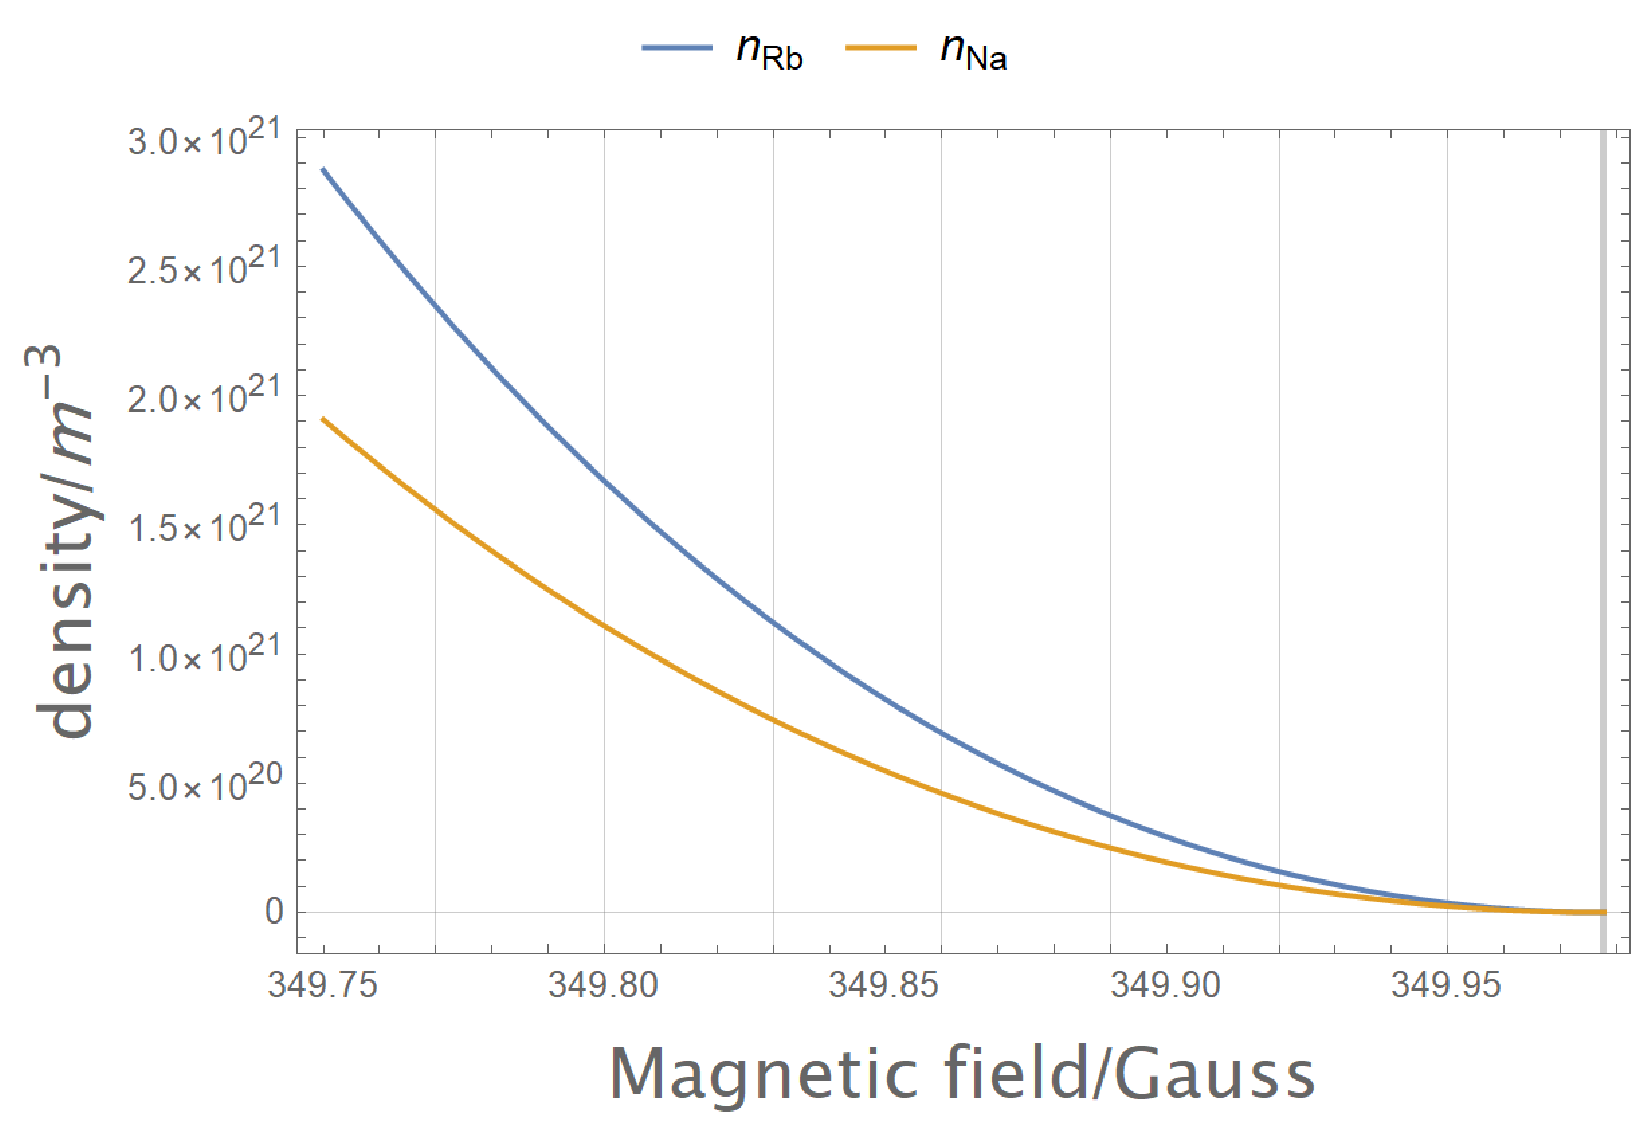
\includegraphics [width = 0.8 \linewidth]{droplet_density.pdf}
\end{center}
\caption[Droplet density as a function of $\delta g$]{Calculated droplet density as a function of $\delta g$. The gray vertical line at the right side shows the zero density boundary. The possible window of magnetic field is around 349.8 Gauss. More details about the Feshbach resonance can be found in Chap. \ref{Chap_Feshbach} and Chap. \ref{Chap_droplet}.}
\label{density-delta_g}
\end{figure}

% homogeneous or in-homogeneous (done 2021-10-28 13:32:03)
The discussion here does not involve the kinetic energy term because we are considering a homogeneous sample, which means that the density of the sample is uniform. However, the actual quantum droplet must be limited in size. Thus, there will be a boundary, and this boundary will bring kinetic energy. This kinetic energy plays a decisive role in the occurrence of liquid-gas phase transition under a specific delta g. The details will be discussed in Chap. \ref{Chap_droplet}. What needs to be reminded here is that the density calculated here does not take into account the constraints of surface tension caused by kinetic energy. It will be slightly lower than the density in the real experimental sample. Of course, if it is an extensive droplet sample, this difference can be ignored.

\chapterend

